\chapter{Discussion} \label{ch:discussion}
A discussion of the test is given in this chapter. The main focus is to discuss the system's capability to be supportive of natural language control. The three common errors of the test actions given in the previous chapter are used to discuss the system's natural language interpretation skills. Therefore, the first three sections are about the errors, while the last sections are a discussion of the system as a whole regarding the subject of natural language control.


\section{Error when not specifying axis direction}
Given the graph in figure \ref{fig:error} in the previous chapter, it is seen that the most common error is using the term 'up' to describe a movement in the z-axis. An example from the dataset is \textit{"move 10 centimeters up"}. The system would be able to interpret a movement of 0.1 meters, but not in what direction. The adverb meaning of 'up' does not refer to any direction in the system.
The words 'up' and 'down' require the robot to know how the user perceives the environment. It is therefore difficult to know what direction is meant and, therefore, how the words should be processed.
It is possible to assign the word 'up' as a synonym for the z-axis of the work frame, but that would not guarantee a correct interpretation. Figure \ref{fig:TCP_axis} shows that the z-axis points directly downward. In this particular system, 'up' should be interpreted as a negative z-axis movement.


\begin{figure}[ht]
    \centering
    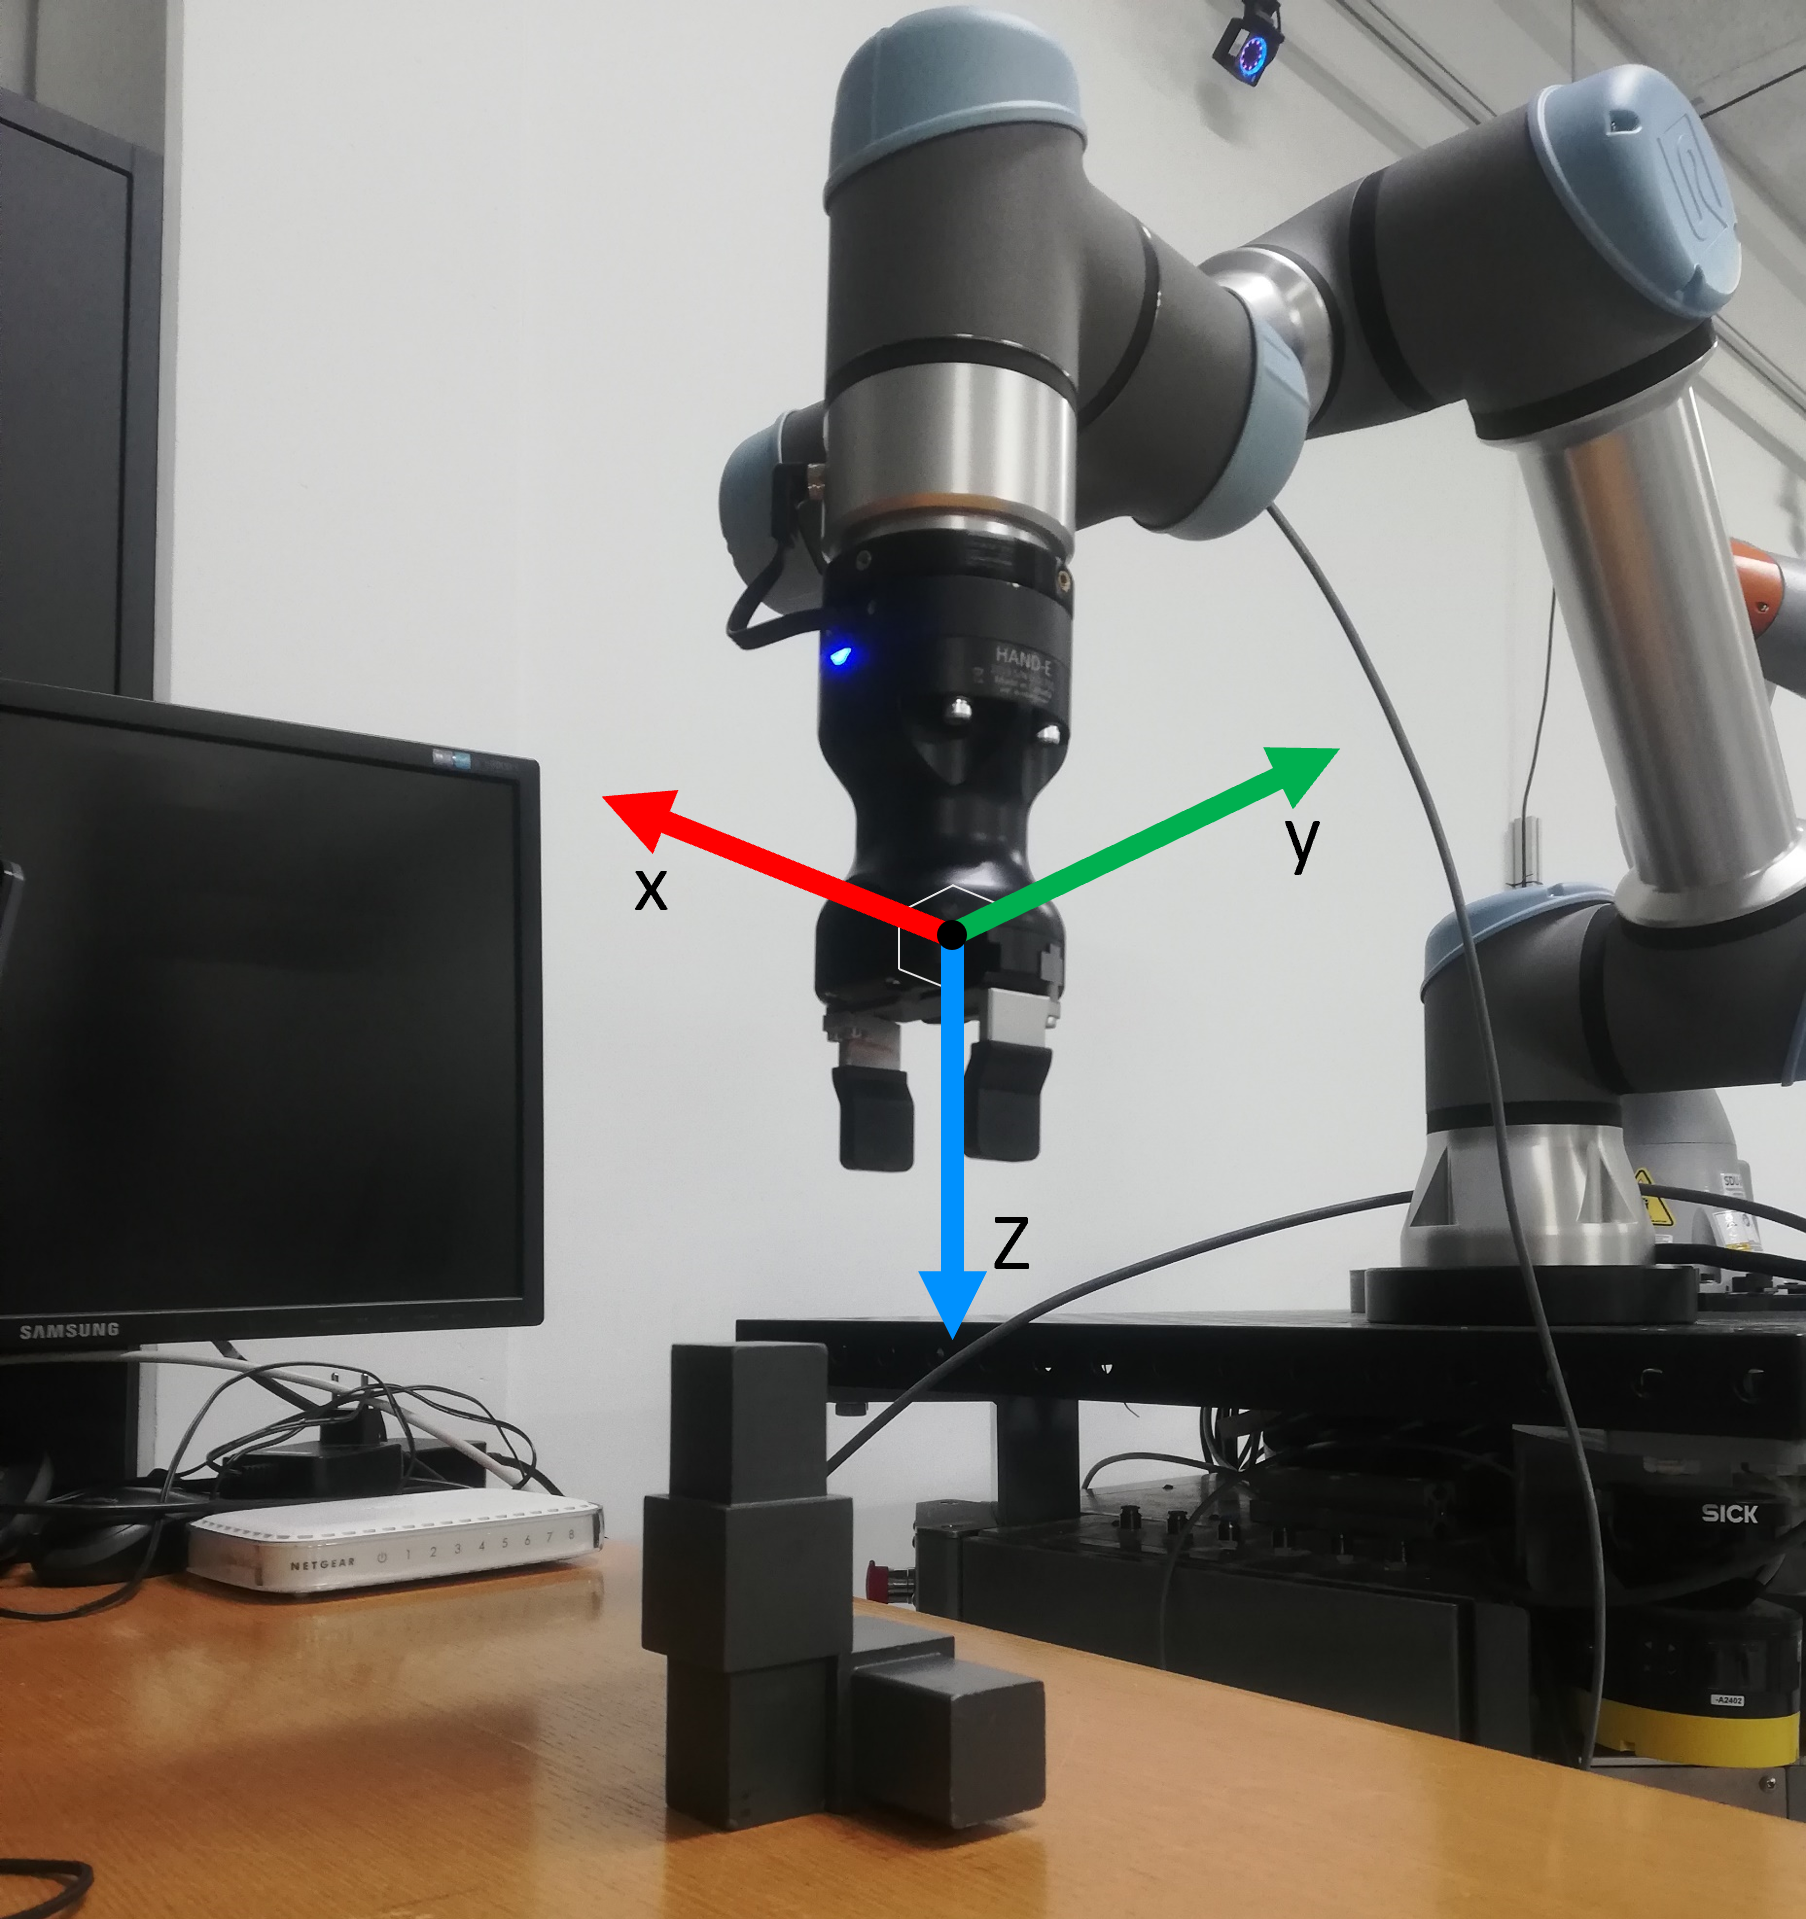
\includegraphics[width=9cm]{img/axis_of_TCP_frame.png}
    \caption{Figure showing the axis of the TCP frame in the given work environment.}
    \label{fig:TCP_axis}
\end{figure}

And if 'up' was assigned as a negative z-axis movement, then another TCP frame could be imagined where that would also be incorrect.
Even if it was assigned to the z-axis of the base frame of the robot (which points upwards in reference to gravity, given the robot is mounted horizontally), then an environment could be imagined where the z-axis of the base frame was not pointing upwards in the workspace of the robot TCP. Figure \ref{fig:exception_frame_TCP} shows a task where a robot is working on a skewed wooden plank. In this case, upwards is arguably the direction of the z-axis on the TCP frame instead.

\begin{figure}[ht]
    \centering
    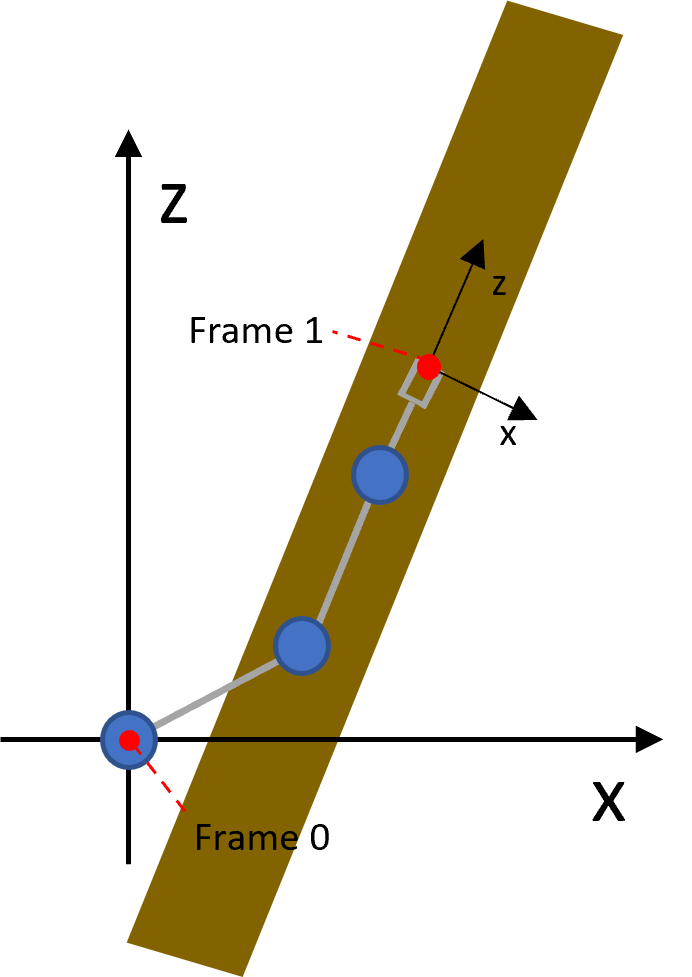
\includegraphics[width=6cm]{img/example_up_in_workspace.png}
    \caption{Figure of a robot doing arbitrary work on a skewed wooden plank.}
    \label{fig:exception_frame_TCP}
\end{figure}
A possible fix is to make the system ask users what direction was meant and temporarily save it while working on the current frame. But this would make the system harder to control, as it could potentially force users to work using 3-dimensional vectors. It would be tedious if one had to specify an instruction as \textit{'move 10 centimeters up, and up is the direction of the vector (x=0.48, y = 0.64, z = 0.6)'}. This type of ambiguous language is therefore left uninterpretable.

\section{Errror made by the POS tagger}
Another error is the POS-tag error. This is an NLP pipeline error where the words are assigned the incorrect grammatical categories. Examples of this error are shown in figure \ref{fig:POS_TAG_ERROR}. The instruction in subfigure 8.3.a is intended to make the system do the gripping maneuver with its arm. Technically, the NLP pipeline is not wrong, as it could also be read as the object being a 'computer grip'. Subfigure 8.3.b is less intuitive but still correct. The system perceives it as the user telling the robot that there is a gripper close by. Instead of the user instructing the robot to close its gripper. Since the key verbs are perceived as nouns, they go undetected by the parser pipeline and are therefore uninterpretable by the system. This cannot be fixed quickly, as it would require training the language model on a new dataset, which would make the language model prone to looking at sentences as instructions. This would be a time-consuming task, which is why it is left as it is.

\begin{figure}[ht]
    \centering
    \begin{subfigure}[b]{9cm}
        \centering
        
\includegraphics[width=4cm]{img/POS_tag_error.png}
        \caption{$ $}
        \label{fig:POS_error_1}
    \end{subfigure}
    \begin{subfigure}[b]{9cm}
        \centering
        
\includegraphics[width=6.5cm]{img/robot_close_gripper_POS_error.png}
        \caption{$ $}
        \label{fig:POS_error_2}
    \end{subfigure}

       \caption{Figure of two tables, where the upper words are instruction words, and the lower words are the grammatical categories assigned by the NLP pipeline.}
       \label{fig:POS_TAG_ERROR}
\end{figure}


The POS tagger is still greater than a simple word detector, as it gives the correct grammatical tags to words with many meanings. The word 'point' has been used throughout the thesis as a location in space, but it could also be perceived as a verb. The POS tagger can then be used to analyze the sentence given in figure \ref{fig:POS_COOL}. The verb is then used to instruct the robot, and the noun is used as the destination. It should be noted that the sentence serves as an example and that the system is not capable of orienting itself towards points, as indicated.

\begin{figure}[ht]
    \centering
    
\includegraphics[width=12cm]{img/POS_is_cool_i_swear.png}
    \caption{Figure of a sentence where the word 'point' is used for two different meanings.}
    \label{fig:POS_COOL}
\end{figure}

\section{Error made when using other words instead of points}
The last error is the use of alternative names instead of points to move to positions. An example from the data is the instruction \textit{'go back to the starting position'}. In this instruction, it is unknown for the system where the 'starting position' is located. A fix to this problem might be to assign names to the points at creation so the user has the ability to call the points by the names set. This would, however, require the system to support movements to destinations specified by arbitrary names. This is not supported by the system, as the parser pipeline only creates move actions to destinations given as nouns (points and frames). Setting up a system that could support point naming would then require a new iteration of the system parser pipeline, where the instruction could contain an arbitrary name that the parser pipeline had to detect. An example of why this task is so difficult could be if one were to name a point 'move'. The parser pipeline would then have to be able to interpret the word 'move' as a point and not as a verb while knowing that the verb 'move' sometimes also correlates to the 'move' action. This is the reason why the given event is left uninterpretable.

\section{limitations}
This section explains the overall limitations which are observed within the system given the test evaluation. It is shown that the system has a clear lack ability of to interpret context-based information. This limitation comes from the design of the parser pipeline, as it can only parse a limited set of formulations. Furthermore, the system fails to interpret some inputs, as it relies on the language model to deliver the correct information. Therefore, if the language model fails, for any reason, then it would likely mean, that the rest of the pipeline would fail as well.
A limitation of the action design created is the limited amount of information passed from the parser into the kinematics pipeline. It is possible to expand the complexity of each instruction. But the parser pipeline would also become increasingly complex, as it would need to extract more information from the language model.
\\\\
The limitations explained, mostly reside within the parser pipeline, where it is observed that the extraction method is insufficient, as it cannot interpret all commands given by the test users. Solutions to the issue, unbound by the structure and design of natural language processing in this thesis, include using self-trained neural networks to map commands into the actions themselves. This method has the feature, that the language used by the test users is directly trained on to gain the actions needed. A method for foreseeing the input structure and processing it would then become unnecessary. In theory, all context-based commands would then be mapped to the actual actions, given that the system is trained enough to interpret the input. The main drawback of this method is the lack of datasets. Given the niche field of using Natural Language to control a 6-DOF manipulator with a parallel gripper, there is little training data available. Training data would therefore be needed to be developed by hand. Another drawback is also the lack of flexibility, as the system would be bound to the actions present at the training. Developing new actions would then require new training in the system. Assuming available training data, it would be possible to train the system to become greater at interpreting the natural language commands given in the test evaluation.


\section{Evaluation of natural language support}
The test users were observed to prefer natural names for points and adverbs to describe relative movements. Some also did not specify movement distance and instead used instructions like 'textit{move up}' or '\textit{move away from the block}'.
The analysis of the errors from the test results also shows that most of the errors stem from the user specifying the instructions using words regarding the work environment like '\textit{move up to the initial height}' or '\textit{go back to the starting position}'. As the specification could mean different positions given interpretation, the system is not capable of interpreting the instructions.
Excluding moving relatively, then the system has good test results interpreting actions that did not need detailed specification, like '\textit{open the gripper}', or '\textit{move to point 0}'. Where good test results mean around 70\% success rate.
